\section{Accelerometer} 
Et accelerometer er et elektromekanisk apparat som anvendes til at måle accelerationskræfter. Det kan blandt andet registrere om et objekt bevæges opad eller nedad samt måle lineær acceleration\citep{Goodrich2013}. Enheden måles i meter per sekund i anden($m/s^2$) eller i g-kræfter (g). En g-kraft på jorden svarer til tyngdekræften på 9,8 $m/s^2$ , men varierer med elevation. \citep{Sparkfun}
Hvis accelerometeret vender opad, vil outputtet være +1 g. Tilsvarende vil accelerometerets output være -1 g hvis det vender nedad, og 0g hvis det er horisontalt. Accelerometerts retninger illustreres på \figref{fig:g}. \citep{Instruments}

\begin{figure}[H]
	\centering
	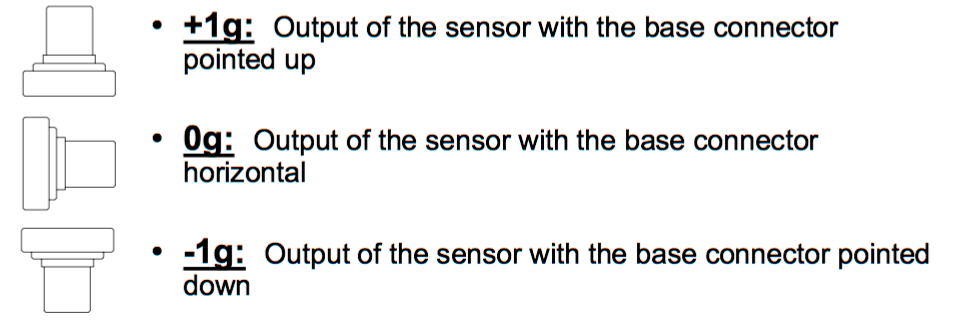
\includegraphics[scale=0.25]{figures/bProblemloesning/g.png}
	\caption{På figuren ses outputtet i g afhængigt af retning på accelerometeret. \citep{Instruments}}
	\label{fig:g}
\end{figure}

Et accelerometer måler to former for acceleration: statisk og dynamisk. De statiske kræfter er tyngdekraften og  vinkelretning af accelerometeret. De dynamiske kræfter er hvilken retning acceleromeret bevæges og dets vibrationer. \citep{Sparkfun,Engineering, Goodrich2013}

%Et accelerometer kan kobles til AC og DC forsyninger. Et AC-koblet accelerometer kan ikke måle statiske accelerationer, men kun dynamiske accelerationer og har derfor ikke ligeså mange funktioner som et DC-koblinger som kan måle både statiske og dynamiske accelerationer.  \citep{Chu}
 

 Acceleration kan måles i flere retninger ved brug af mere end et accelerometer. \citep{Sparkfun}. kan måle acceleration af en akse, to akser(x,y) og tre akser (x,y,z) For eksempel har en bil to akser og de fleste smartphones har 3 akser. \citep{Sparkfun}
 De mest anvendte accelerometre er den piezoelektriske effekt og den kapacitance sensor. 

Den piezoelektriske effekt er den mest almindelige form for accelerometer. Denne anvender mikroskopiske krystalstrukturer, som stresses på grund af accelererende kræfter. Krystallerne danner en spænding ud fra stressen, hvor accelerometeret anvender denne spænding til at bestemme hastighed og retning. \citep{Goodrich2013}

Det kapacistanse\fxnote{Kapacitans er et mål for, hvor meget elektrisk ladning som gemmes (eller separeres) for en given elektrisk spændingsforskel} accelerometer, registrerer når der forekommer ændringer i kapacistans mellem mikrostrukturer, som er ved siden af enheden. Hvis en accelererende kraft får en af disse strukturer til at bevæges, så vil kapacitansen registere ændringen og accelerometeret vil oversætte denne kapacitans som en spænding.  \citep{Goodrich2013}
